% Chapter 4
\chapter{ĐỀ XUẤT HỆ THỐNG DT-GUARD}
\label{Chapter4}

Chương này mô tả kiến trúc DT-Guard, khung phòng thủ chủ động cho FL trong IoT IDS. Nội dung gồm: phát biểu bài toán, kiến trúc tổng thể, bộ sinh dữ liệu thách thức, pipeline kiểm định 4 lớp, cơ chế DT-PW với Effort Gate, và phân tích lý thuyết.

\section{Phát biểu bài toán và ý tưởng cốt lõi}

\subsection{Phát biểu bài toán phòng thủ trong FL-IDS}
Xét hệ thống FL-IDS gồm N client $\{C_{1}, C_{2}, \ldots, C_{N}\}$ cùng huấn luyện một mô hình phát hiện xâm nhập toàn cục $\mathbf{w}$ qua R vòng lặp. Trong đó, tập client bao gồm N - K client lành tính (tập B) và K client độc hại (tập M), với K không biết trước. Mỗi client i sở hữu tập dữ liệu cục bộ $D_{i}$ có phân phối Non-IID theo Dirichlet($\alpha)$.

Bài toán phòng thủ được phát biểu:

\textbf{Đầu vào:} Tại mỗi round t, server nhận tập bản cập nhật $\{\mathbf{w}_{1}^{(t)}, \mathbf{w}_{2}^{(t)}, \ldots, \mathbf{w}_{N}^{(t)}\}$ từ N client. Server có quyền truy cập mô hình toàn cục $\mathbf{w}^{(t-1)}$ của round trước nhưng không có quyền truy cập dữ liệu thô $D_{i}$ của bất kỳ client nào.

\textbf{Đầu ra mong muốn:} (1) Mô hình toàn cục $\mathbf{w}^{(t)}$ duy trì Accuracy cao bất chấp sự hiện diện của tập M; (2) Phát hiện và loại bỏ chính xác client thuộc M: Detection Rate (DR) cao, False Positive Rate (FPR) thấp; (3) Trọng số tổng hợp $w_{i}$ phản ánh đúng mức đóng góp tri thức thực tế, gán $w_{i}$ = 0 cho free-rider.

\textbf{Ràng buộc:} (1) Không truy cập dữ liệu thô, server chỉ thấy tham số mô hình; (2) Overhead tính toán phải nhỏ hơn 1\% tổng thời gian mỗi round; (3) Hoạt động hiệu quả trên nhiều loại tấn công (Backdoor, LIE, Min-Max, Min-Sum, MPAF) và nhiều tỉ lệ K/N (10\%--50\%).

\subsection{Ý tưởng cốt lõi: Kiểm chứng hành vi chủ động}
Như đã phân tích trong Chương 2, nguyên nhân gốc rễ của ba khoảng trống nghiên cứu nằm ở cách tiếp cận phân tích tham số thụ động: tất cả các phương pháp phòng thủ hiện có đều chỉ phân tích đặc trưng tĩnh của tham số mô hình mà không kiểm chứng hành vi suy luận thực tế.

DT-Guard đề xuất chuyển từ \textbf{passive parameter inspection} sang \textbf{active behavioral verification}: thay vì chỉ đánh giá hình thái tham số, server chủ động kiểm chứng năng lực suy luận của mô hình trên dữ liệu kiểm thử được kiểm soát. Cách tiếp cận này dựa trên hai \textbf{giả thuyết khoa học} sau:

\textbf{Giả thuyết H1 (Client Non-IID lành tính):} Client i $\in$ B có dữ liệu $D_{i}$ thiên lệch về một số lớp sẽ có tham số $\mathbf{w}_{i}$ lệch xa mô hình toàn cục $\mathbf{w}$. Các phương pháp thụ động (Krum, GeoMed, LUP) đo $\|\mathbf{w}_{i} - \mathbf{w}\|_{2}$ và dễ nhầm đây là tấn công, gây FPR cao. Tuy nhiên, khi được kiểm tra trên dữ liệu thách thức cân bằng nhãn $D_{\text{ch}}$, mô hình vẫn phân loại chính xác, vì client đã thực sự học được tri thức hữu ích từ dữ liệu riêng.

\textbf{Giả thuyết H2 (Tấn công tối ưu ngược):} Client j $\in$ M sử dụng LIE {[}1{]}, Min-Max/Min-Sum {[}15{]} có thể giữ $\mathbf{w}_{j}$ trong vùng phân phối thống kê bình thường ($\|\mathbf{w}_{j} - \mathbf{w}\|_{2}$ nhỏ), khiến các phương pháp thụ động không phát hiện được. Tuy nhiên, khi buộc phải phân loại trên $D_{\text{ch}}$, mô hình sẽ bộc lộ hành vi sai: F1 thấp trên các lớp tấn công.

Digital Twin đóng vai trò môi trường kiểm thử cách ly (sandbox) tại phía server để thực hiện kiểm chứng này một cách an toàn và tách biệt. Cách tiếp cận này cho phép server kiểm chứng từng mô hình trước khi chấp nhận, thay vì chỉ suy luận từ tham số.

\subsection{Ký hiệu toán học}

\begin{longtable}[]{@{}
  >{\raggedright\arraybackslash}p{(\linewidth - 2\tabcolsep) * \real{0.1547}}
  >{\raggedright\arraybackslash}p{(\linewidth - 2\tabcolsep) * \real{0.7733}}@{}}
\caption{Bảng tổng hợp các ký hiệu toán học chính} \\
\toprule\noalign{}
\begin{minipage}[b]{\linewidth}\centering
\textbf{Ký hiệu}
\end{minipage} & \begin{minipage}[b]{\linewidth}\centering
\textbf{Ý nghĩa}
\end{minipage} \\
\midrule\noalign{}
\endfirsthead
%
\multicolumn{2}{c}{{\textit{(tiếp) Bảng 4.1}}} \\
\toprule\noalign{}
\begin{minipage}[b]{\linewidth}\centering
\textbf{Ký hiệu}
\end{minipage} & \begin{minipage}[b]{\linewidth}\centering
\textbf{Ý nghĩa}
\end{minipage} \\
\midrule\noalign{}
\endhead
\bottomrule\noalign{}
\endlastfoot
N & Số client tổng cộng \\
K & Số client độc hại \\
$\mathbf{w}^{(t)}$ & Tham số mô hình toàn cục tại round t \\
$\mathbf{w}_{i}^{(t)}$ & Tham số mô hình cục bộ của client i tại round t \\
$D_{\text{ch}}$ & Bộ dữ liệu thách thức (challenge data) \\
M & Số mẫu trong $D_{\text{ch}}$ \\
L & Số lớp (layer) trainable trong mô hình \\
$s_{i}(ids)$ & IDS Performance Score của client i \\
$s_{i}(param)$ & Parameter Similarity Score của client i \\
$\Delta_{i}^{(t)}$ & Mức lệch tham số chuẩn hóa của client i \\
$T_{i}$ & Trust-Score tổng hợp của client i \\
$d_{i}$ & Prediction divergence của client i \\
$P_{i}$ & Performance-Score của client i \\
$w_{i}$ & Trọng số tổng hợp cuối cùng của client i \\
A & Tập client được chấp nhận (qua cả Trust Gate và Effort Gate) \\
\end{longtable}

\section{Kiến trúc tổng thể DT-Guard}

\subsection{Kiến trúc ba thực thể}
DT-Guard được thiết kế với ba thực thể chính, tách biệt về chức năng và vị trí triển khai:

\textbf{IoT Clients (Tầng cạnh):} Các thiết bị IoT hoặc edge node thực hiện huấn luyện cục bộ trên dữ liệu riêng $D_{i}$ và gửi bản cập nhật $\mathbf{w}_{i}^{(t)}$ về server. Mỗi client sử dụng optimizer Adam với learning rate = $10^{-3}$, batch size 512, huấn luyện E = 3 local epoch mỗi round. Loss function là Weighted Cross-Entropy để xử lý mất cân bằng lớp. Trong thiết lập thực nghiệm, hệ thống gồm 20 client với phân bổ dữ liệu Non-IID theo Dirichlet ($\alpha$ = 0,5).

\textbf{FL Server (Tầng trung tâm):} Server trung tâm điều phối toàn bộ quy trình FL. Server nhận bản cập nhật từ client, chuyển tiếp sang DT Verification Environment để kiểm chứng, nhận kết quả Trust-Score và Performance-Score, thực hiện tổng hợp mô hình toàn cục, và phân phối lại cho client. Server lưu trữ mô hình toàn cục $\mathbf{w}^{(t)}$ và lịch sử kiểm chứng của từng client.

\textbf{DT Verification Environment (Tầng kiểm chứng):} Môi trường kiểm chứng Digital Twin, được tách biệt khỏi FL Server chính. Việc tách biệt cung cấp ba lợi ích: (1) Cách ly hành vi độc hại: mô hình độc hại chạy trong sandbox không ảnh hưởng đến vòng lặp FL chính, vì sandbox sử dụng bản sao tham số và tài nguyên riêng; (2) Kiểm chứng song song: server có thể khởi tạo nhiều DT instance để kiểm tra nhiều client đồng thời, giúp giảm tổng thời gian verification khi số client lớn; (3) Tách biệt verification khỏi aggregation: quy trình kiểm chứng không ảnh hưởng đến thread tổng hợp chính, giữ cho server luôn responsive.

Hình 4.1 trình bày kiến trúc tổng quát của DT-Guard với ba thực thể và luồng tương tác giữa chúng. Ở cấp độ tổng quát, mỗi vòng FL diễn ra như sau: các client gửi bản cập nhật lên FL Server (1); server chuyển tiếp sang DT Verification Environment để kiểm chứng (2); bản cập nhật đạt chuẩn được tổng hợp (3), mô hình toàn cục mới được trả về server (4) và phân phối lại cho client (5). Toàn bộ logic đánh giá (từ sinh dữ liệu thách thức, kiểm định hành vi, đến chấm điểm đóng góp) đều nằm bên trong DT Verification Environment.

\begin{figure}[H]
    \centering
    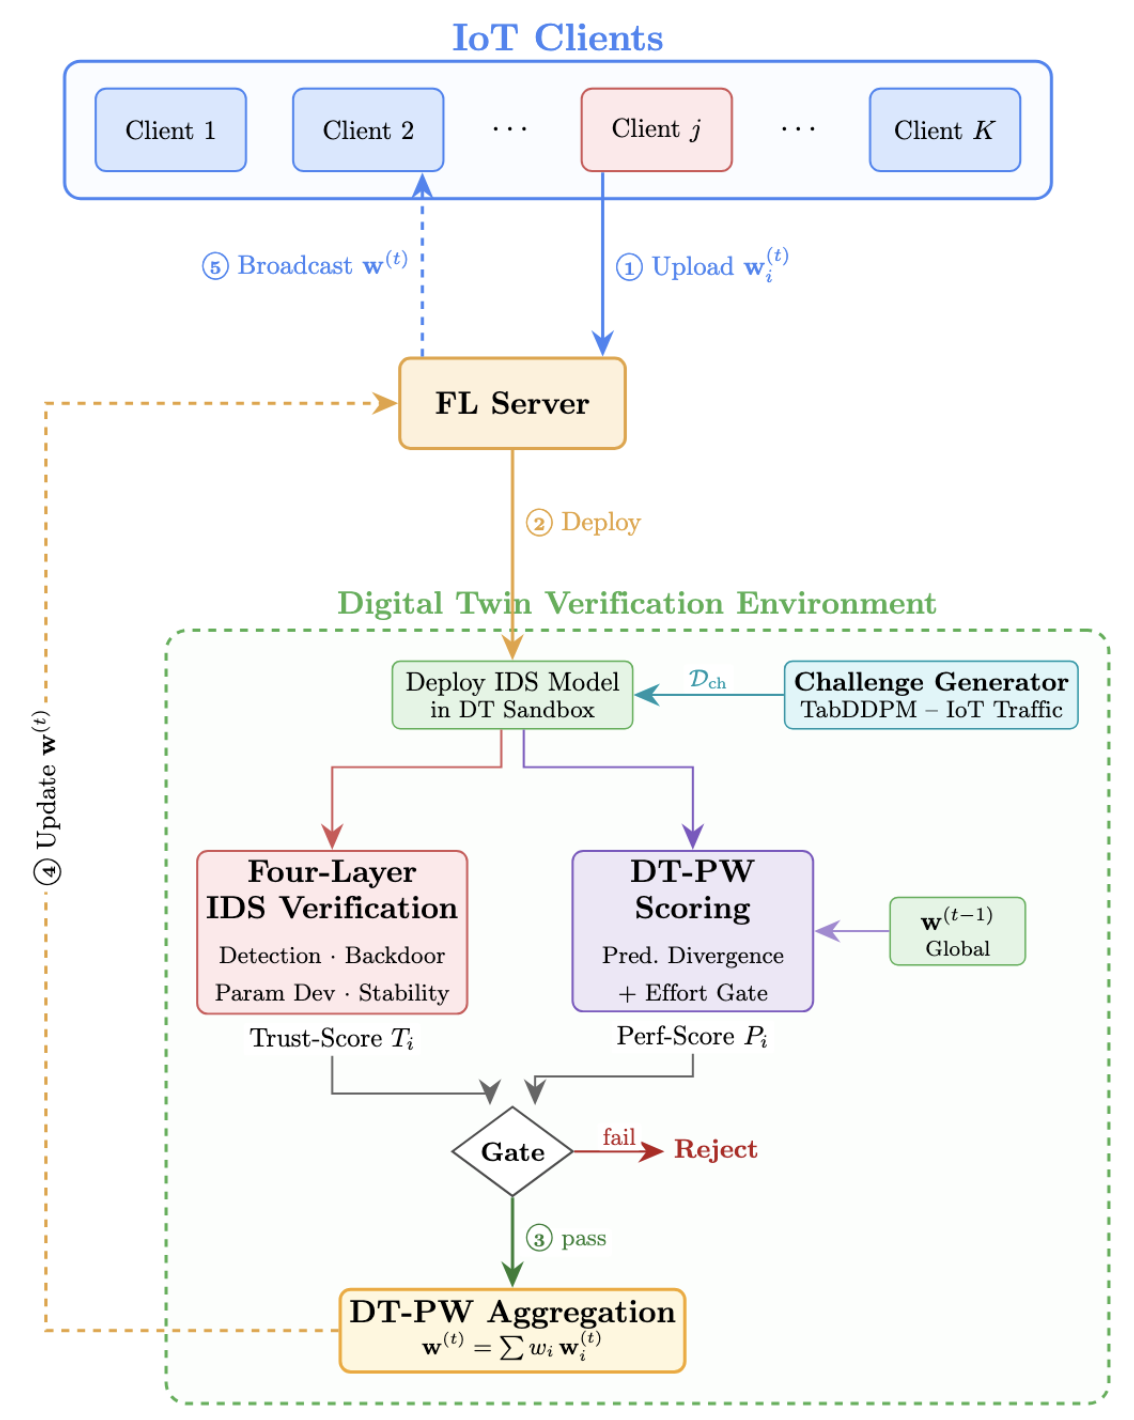
\includegraphics[width=0.85\linewidth]{Figures/fig_4_1_kien_truc_tong_quat_dtguard.png}
    \caption{Kiến trúc tổng quát DT-Guard}
\end{figure}

Phần tiếp theo sẽ đi sâu vào bên trong DT Verification Environment, thành phần cốt lõi tạo nên sự khác biệt của DT-Guard so với các phương pháp hiện có.

\subsection{Cấu trúc bên trong DT Verification Environment}
\begin{figure}[H]
    \centering
    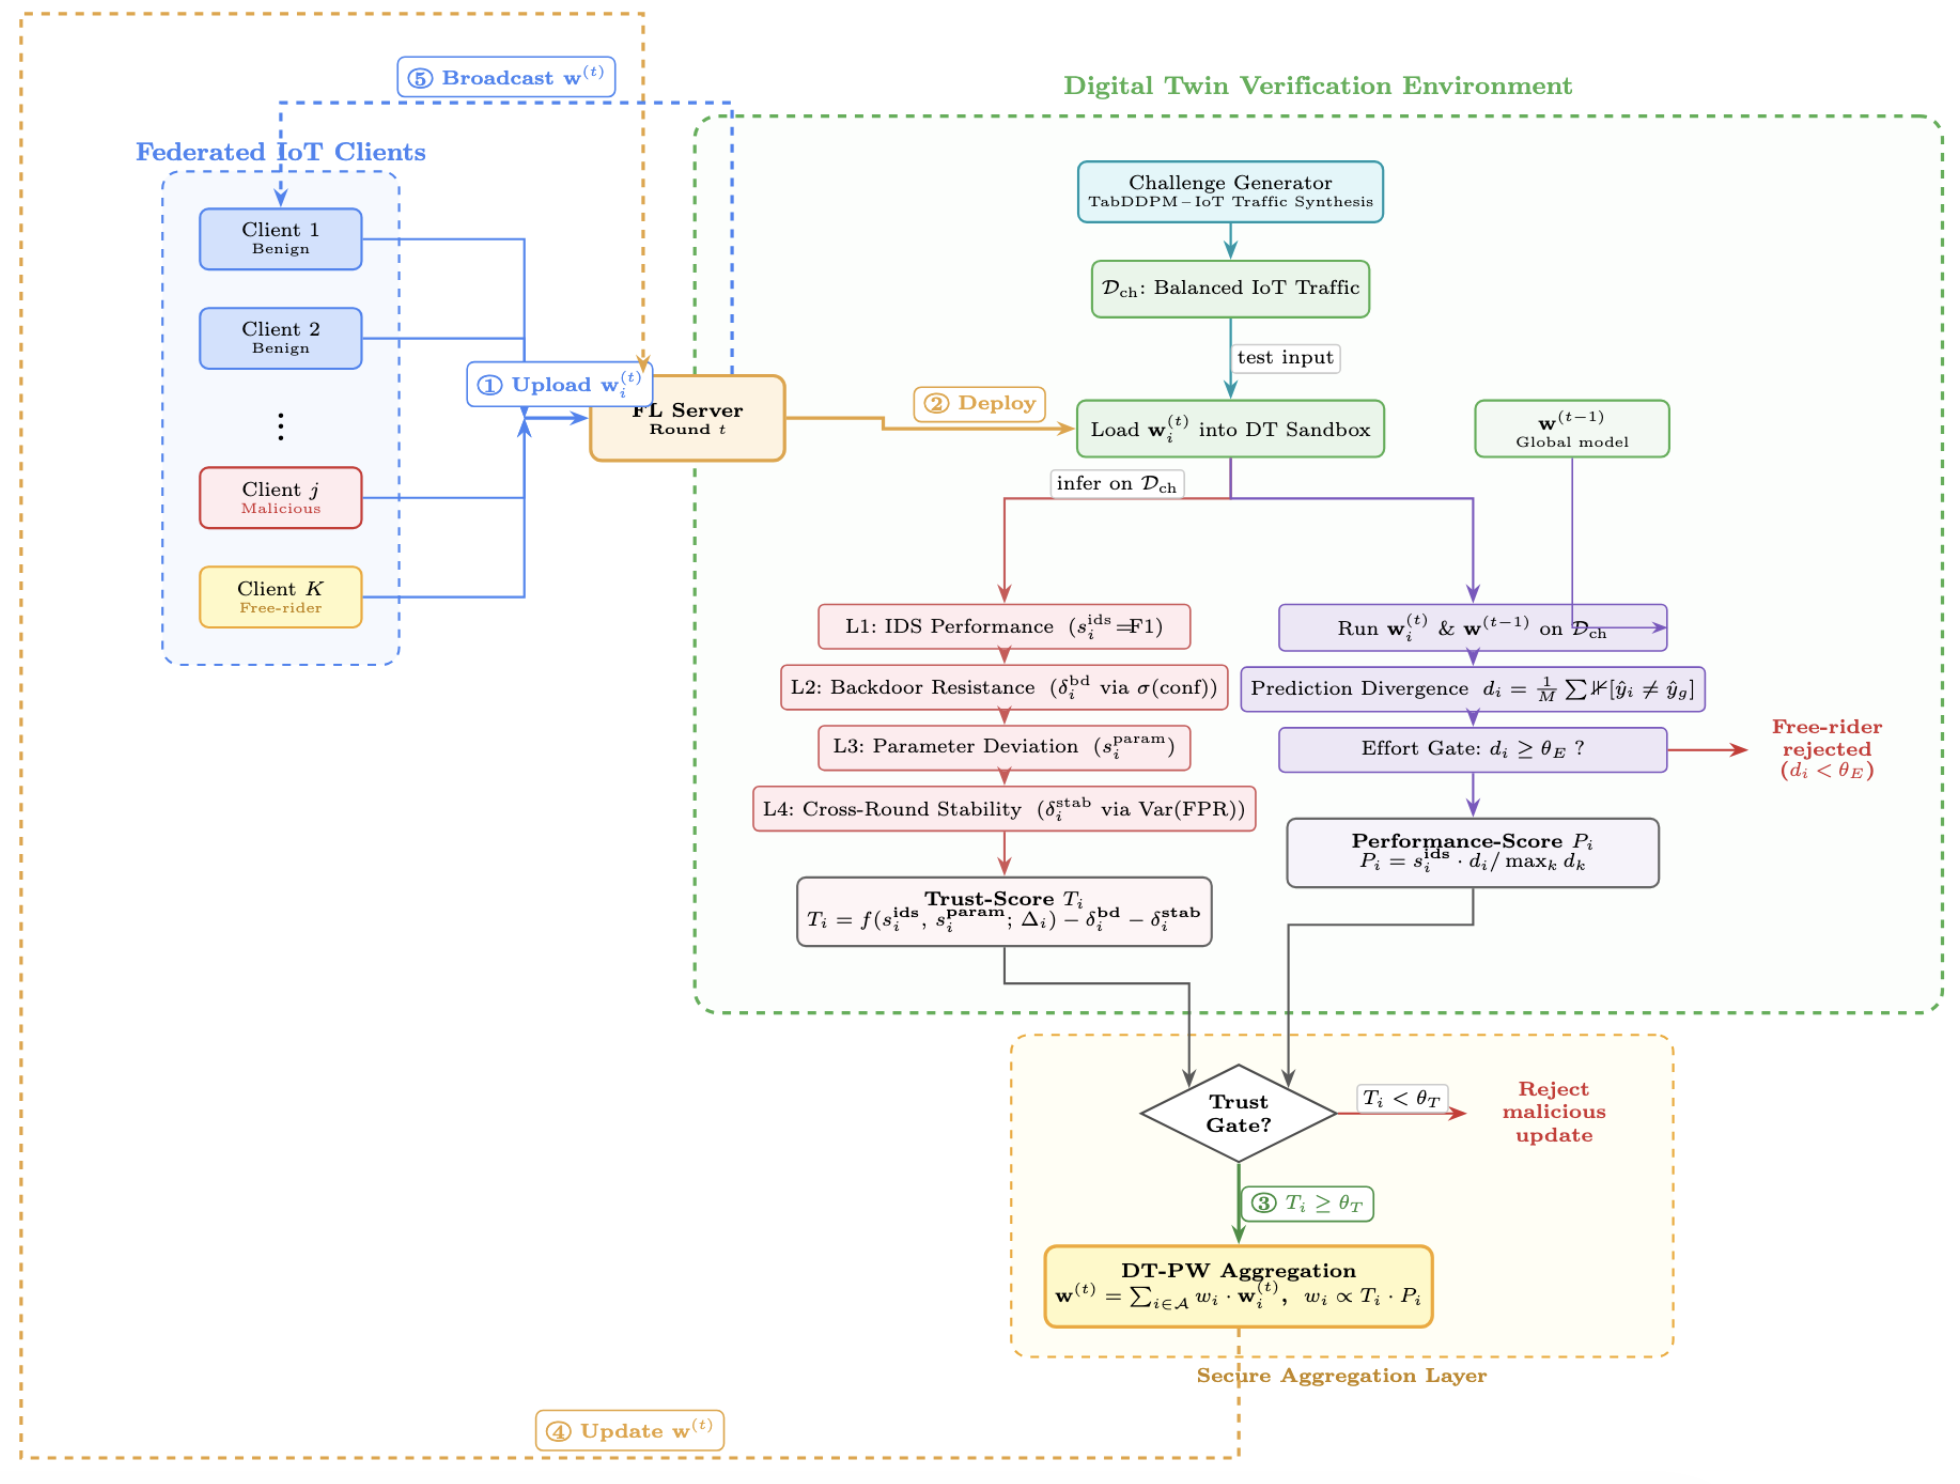
\includegraphics[width=0.85\linewidth]{Figures/fig_4_2_kien_truc_dt_verification_environment.png}
    \caption{Kiến trúc chi tiết DT Verification Environment}
\end{figure}

DT Verification Environment được tổ chức thành bốn tầng xử lý nối tiếp nhau. Mỗi bản cập nhật $\mathbf{w}_{i}^{(t)}$ từ client đi qua lần lượt các tầng này trước khi được chấp nhận hoặc loại bỏ.

Tầng sinh dữ liệu: Challenge Generator. Đây là tầng trên cùng, chịu trách nhiệm cung cấp dữ liệu kiểm thử cho toàn bộ quy trình phía dưới. Challenge Generator sử dụng TabDDPM {[}7{]} để sinh tập $D_{\text{ch}}$ (bao gồm cả lưu lượng bình thường lẫn nhiều dạng tấn công) khác nhau, với phân bổ nhãn cân bằng. Dữ liệu này đóng vai trò "đề thi" mà mọi mô hình cục bộ phải vượt qua. $D_{\text{ch}}$ được sinh trước và lưu sẵn (pre-generated pool), nên không tạo thêm độ trễ trong mỗi vòng FL.

Tầng cách ly: DT Sandbox. Khi FL Server chuyển một bản cập nhật $\mathbf{w}_{i}^{(t)}$ sang DT Environment, bản cập nhật này được nạp vào một sandbox tách biệt. Sandbox chỉ làm việc với bản sao tham số, không sử dụng tham số gốc; mỗi lần chỉ nạp một mô hình rồi giải phóng trước khi nạp mô hình tiếp theo; và được reset về trạng thái sạch sau mỗi lần kiểm chứng. Thiết kế này đảm bảo mô hình độc hại không thể ảnh hưởng đến server hay các mô hình khác.

Từ sandbox, quá trình đánh giá phân thành hai nhánh song song, mỗi nhánh giải quyết một bài toán riêng biệt:

Nhánh thứ nhất: Four-Layer Verification Pipeline. Nhánh này trả lời câu hỏi: \emph{"Mô hình này có đáng tin hay không?"} Mô hình được chạy trên $D_{\text{ch}}$ rồi đánh giá qua bốn lớp kiểm định liên tiếp: (L1) hiệu năng phát hiện xâm nhập, (L2) khả năng kháng backdoor, (L3) mức lệch tham số so với mô hình toàn cục, và (L4) độ ổn định hành vi qua các vòng. Bốn điểm thành phần được tổng hợp thành một Trust-Score $T_{i}$ duy nhất. Chi tiết từng lớp được trình bày tại Mục 4.4.

Nhánh thứ hai: DT-PW Scoring. Nhánh này trả lời câu hỏi: \emph{"Mô hình này có đóng góp tri thức mới hay không?"} Cả mô hình cục bộ $\mathbf{w}_{i}^{(t)}$ lẫn mô hình toàn cục $\mathbf{w}^{(t-1)}$ đều được chạy trên cùng $D_{\text{ch}}$, rồi so sánh kết quả dự đoán của chúng. Mức khác biệt trong dự đoán (gọi là prediction divergence $d_{i})$ phản ánh lượng tri thức mới mà client mang lại. Nếu $d_{i}$ quá thấp (dự đoán gần như trùng khớp với mô hình toàn cục), Effort Gate xác định đó là free-rider và gán điểm đóng góp bằng không. Client vượt qua Effort Gate được chấm Performance-Score $P_{i}$. Chi tiết được trình bày tại Mục 4.5.

Tầng quyết định (Decision Gate). Kết quả từ hai nhánh (Trust-Score $T_{i}$ và Performance-Score $P_{i})$ hội tụ tại đây. Tầng này thực hiện hai bước lọc tuần tự: trước hết, client có $T_{i}$ dưới ngưỡng tin cậy $\theta_{T}$ bị loại bỏ (bản cập nhật bị từ chối); tiếp theo, trong số các client còn lại, những client đã bị Effort Gate đánh dấu là free-rider ($P_{i}$ = 0) cũng bị gán trọng số bằng không. Tập client cuối cùng vượt qua cả hai bộ lọc gọi là $\mathcal{A}$.

Tầng tổng hợp (DT-PW Aggregator). Chỉ các bản cập nhật thuộc tập $\mathcal{A}$ mới tham gia vào việc tổng hợp mô hình toàn cục mới. Trọng số của mỗi client được tính bằng tích $T_{i}$ $\cdot$ $P_{i}$ (chuẩn hóa), đảm bảo client nào vừa đáng tin vừa đóng góp nhiều tri thức mới sẽ có ảnh hưởng lớn nhất. Mô hình toàn cục mới $\mathbf{w}^{(t)}$ sau đó được chuyển ngược lại FL Server.

\subsection{Lý do thiết kế hai nhánh song song}
Việc tách quá trình đánh giá thành hai nhánh độc lập xuất phát từ nhận định rằng hai bài toán (phát hiện client độc hại và phát hiện free-rider) có bản chất khác nhau và không thể giải bằng cùng một chỉ số.

Client độc hại cố tình phá hoại mô hình toàn cục, nhưng có thể ngụy trang tham số để trông bình thường. Để phát hiện chúng, cần đánh giá hành vi suy luận thực tế trên nhiều khía cạnh: đó là việc của Four-Layer Pipeline.

Free-rider không phá hoại, nhưng cũng không đóng góp gì: chúng chỉ sao chép mô hình toàn cục rồi gửi lại. Mô hình của free-rider vẫn phân loại đúng (vì bản chất là mô hình toàn cục), nên Four-Layer Pipeline không loại được chúng. Để phát hiện free-rider, cần so sánh dự đoán cục bộ với dự đoán toàn cục: đó là việc của DT-PW Scoring.

Hai nhánh sử dụng chung $D_{\text{ch}}$ làm đầu vào nhưng tính toán độc lập. Trust-Score đánh giá chất lượng tuyệt đối của mô hình, Performance-Score đánh giá mức đóng góp tương đối so với mô hình toàn cục. Chỉ khi kết hợp cả hai qua Công thức (4.11), hệ thống mới đồng thời loại được client độc hại, loại free-rider, và ưu tiên client đóng góp thực chất.

\subsection{Luồng hoạt động 5 bước mỗi vòng FL}
Mỗi vòng FL \emph{t} diễn ra theo năm bước:

\textbf{Bước 1 (Upload).} Mỗi client i nhận mô hình toàn cục $\mathbf{w}^{(t-1)}$ từ server, huấn luyện cục bộ E = 3 epoch trên dữ liệu riêng $D_{i}$ (optimizer Adam, lr = $10^{-3}$, batch size 512, Weighted Cross-Entropy loss), và gửi bản cập nhật $\mathbf{w}_{i}^{(t)}$ về FL Server. Tại thời điểm này, server chưa có thông tin nào về độ tin cậy hay mức đóng góp của từng client.

\textbf{Bước 2 (Deploy).} Thay vì tổng hợp ngay, FL Server chuyển từng $\mathbf{w}_{i}^{(t)}$ sang DT Verification Environment. Mô hình được nạp vào sandbox và chạy inference trên $D_{\text{ch}}$. Hai nhánh đánh giá hoạt động tuần tự: Four-Layer Pipeline tính Trust-Score $T_{i}$; DT-PW Scorer tính prediction divergence $d_{i}$ và Performance-Score $P_{i}$.

\textbf{Bước 3 (Gate \& Aggregate).} Decision Gate kiểm tra hai điều kiện: (a) Trust Gate: nếu $T_{i}$ \textless $\theta_{T}$, bản cập nhật bị từ chối ($\theta_{T}$ = 0,6 cho CIC-IoT-2023, $\theta_{T}$ = 0,5 cho ToN-IoT, được điều chỉnh theo độ phức tạp của từng dataset); (b) Effort Gate: trong số các client còn lại, nếu $d_{i}$ \textless $\theta_{E}$ thì $P_{i}$ = 0 (free-rider). Tập client cuối cùng được chấp nhận là $\mathcal{A}$.

\textbf{Bước 4 (Update).} Mô hình toàn cục mới được tổng hợp: $\mathbf{w}^{(t)}$ = $\sum_{i \in \mathcal{A}} w_{i} \cdot \mathbf{w}_{i}^{(t)}$ với trọng số:

\[w_{i} = \frac{T_{i} \cdot P_{i}}{\sum_{k \in \mathcal{A}}^{}(T_{k} \cdot P_{k})}\]

Kết quả được chuyển ngược lại FL Server.

\textbf{Bước 5 (Broadcast).} FL Server phân phối $\mathbf{w}^{(t)}$ cho tất cả N client để bắt đầu vòng lặp tiếp theo.

\section{Bộ sinh dữ liệu thách thức (Challenge Data Generator)}

\subsection{Vai trò và yêu cầu}
Trong hệ thống FL-IDS, server không có quyền truy cập dữ liệu thô của client. Do đó, để kiểm chứng hành vi mô hình, server cần một bộ sinh dữ liệu (generative model) để tạo ra dữ liệu kiểm thử đại diện, gọi là challenge data $D_{\text{ch}}$. Chất lượng của $D_{\text{ch}}$ quyết định trực tiếp khả năng phân biệt của toàn bộ khung DT-Guard.

$D_{\text{ch}}$ cần đáp ứng bốn yêu cầu:

\textbf{(1) Fidelity (Độ trung thực):} Phân phối dữ liệu tổng hợp phải gần với phân phối dữ liệu thực, đo bằng TSTR (Train on Synthetic, Test on Real), khoảng cách Wasserstein (biến liên tục), và Jensen-Shannon Distance (biến phân loại).

\textbf{(2) Coverage \& Diversity (Bao phủ và đa dạng):} Dữ liệu phải bao phủ đa dạng các lớp lưu lượng, đồng thời các mẫu sinh ra phải đa dạng, tránh mode collapse, đo bằng DCR (Distance to Closest Record) và hệ chỉ số PRDC (Precision, Recall, Density, Coverage).

\textbf{(3) Conditional Control (Kiểm soát điều kiện):} Bộ sinh phải hỗ trợ class-conditional generation (sinh mẫu theo nhãn chỉ định) để tạo $D_{\text{ch}}$ cân bằng nhãn. Đo bằng Label Accuracy qua Oracle classifier.

\textbf{(4) Efficiency (Hiệu quả):} Tốc độ huấn luyện và sinh mẫu phải đủ nhanh để tích hợp vào vòng lặp FL mà không tạo nút thắt, đo bằng Training Time, Generation Latency, và CPU/RAM.

\subsection{A/B Testing chọn mô hình sinh}
Đề tài tiến hành A/B Testing trên năm mô hình sinh dữ liệu dạng bảng thuộc hai họ:

\begin{itemize}
\item
  \textbf{Nhóm Diffusion:} TabDDPM {[}7{]}: MLP denoising, 256 hidden units, SiLU activation, \emph{T} = 200 bước, 100 epoch; TabSyn {[}20{]}: VAE kết hợp latent diffusion, 256 hidden units; ForestDiffusion {[}6{]}: sử dụng XGBoost thay vì neural network để khử nhiễu, chỉ chạy trên CPU.
\item
  \textbf{Nhóm GAN:} CTGAN {[}17{]}: Conditional GAN chuyên biệt dữ liệu bảng, mode-specific normalization, 256 hidden units, 300 epoch; WGAN-GP {[}4{]}: Wasserstein GAN với gradient penalty $\lambda$ = 10, 256 hidden units, 300 epoch.
\end{itemize}

\textbf{Quy trình A/B Testing gồm ba bước:}

\textbf{(Bước 1) Huấn luyện và sinh dữ liệu.} Mỗi mô hình được huấn luyện trên cùng tập dữ liệu seed (một phần dữ liệu mà server nắm giữ, không chứa dữ liệu cục bộ của bất kỳ client nào), đảm bảo điều kiện đầu vào đồng nhất cho so sánh công bằng. Sau khi huấn luyện, mỗi mô hình sinh cùng số lượng mẫu với phân bổ nhãn cân bằng giữa các lớp, tạo ra năm tập dữ liệu tổng hợp $\{\hat{D}_{1}, \hat{D}_{2}, \ldots, \hat{D}_{5}\}$.

\textbf{(Bước 2) Đánh giá theo bốn nhóm tiêu chí.} Mỗi tập dữ liệu tổng hợp $\hat{D}_{i}$ được đánh giá trên cả CIC-IoT-2023 và ToN-IoT qua bốn nhóm tiêu chí:

\begin{itemize}
\item
  \textbf{Fidelity}: dữ liệu tổng hợp phản ánh sát phân phối thực tế đến mức nào. Đo bằng hai chỉ số: TSTR (Train on Synthetic, Test on Real), huấn luyện mô hình phân loại trên $\hat{D}_{i},$ kiểm tra trên dữ liệu thật; TSTR càng cao thì dữ liệu sinh càng sát thực. Wasserstein Distance: khoảng cách giữa phân phối đặc trưng của $\hat{D}_{i}$ và dữ liệu thật; giá trị càng thấp càng tốt.
\item
  \textbf{Coverage \& Diversity}: dữ liệu bao phủ đầy đủ và đa dạng các lớp lưu lượng hay không. Đo bằng Recall (tỷ lệ mẫu thật có ít nhất một mẫu sinh gần tương tự, Recall cao nghĩa là không bỏ sót vùng nào của phân phối thực) và DCR (Distance to Closest Record, khoảng cách từ mẫu sinh đến mẫu thật gần nhất, đảm bảo không trùng lặp).
\item
  \textbf{Conditional Control}: bộ sinh có tạo được mẫu theo nhãn chỉ định chính xác không. Đo bằng Label Accuracy qua Oracle classifier, huấn luyện một mô hình phân loại trên dữ liệu thật, dùng nó kiểm tra nhãn của mẫu sinh; accuracy cao nghĩa là conditional generation hoạt động tốt.
\item
  \textbf{Efficiency}: chi phí tính toán để huấn luyện và sinh mẫu. Đo bằng Training Time (thời gian huấn luyện) và Generation Latency (thời gian sinh một batch).
\end{itemize}

\textbf{(Bước 3) Tổng hợp composite score và lựa chọn.} Bốn nhóm tiêu chí được chuẩn hóa về thang {[}0, 10{]} rồi tổng hợp thành composite score có trọng số bằng nhau. TabDDPM đạt composite score cao nhất (7,3/10) nhờ: TSTR 71,4\% (cao nhất); Wasserstein Distance 0,061 (thấp nhất); Recall 0,98 (gần bao phủ toàn bộ); Training time \textasciitilde200 giây (nhanh gấp $8\times$ CTGAN). Kết quả nhất quán trên cả hai dataset. Chi tiết kết quả A/B Testing tại Mục 5.3.

\subsection{Quy trình sinh dữ liệu thách thức}
Quy trình sinh $D_{\text{ch}}$ được thiết kế để tối ưu hóa giữa chất lượng kiểm thử và chi phí tính toán, gồm ba giai đoạn:

\textbf{(Giai đoạn 1)} Huấn luyện TabDDPM trên dữ liệu seed (thực hiện một lần trước vòng lặp FL): Server sử dụng tập dữ liệu seed (một phần dữ liệu công khai hoặc dữ liệu mà server nắm giữ, \textbf{không} chứa dữ liệu cục bộ của bất kỳ client nào) để huấn luyện mô hình TabDDPM. Cấu hình huấn luyện: kiến trúc MLP với 256 hidden units, activation SiLU, \emph{T} = 200 bước diffusion, 100 epoch. Biến liên tục được xử lý bằng Gaussian diffusion, biến phân loại bằng multinomial diffusion (chi tiết tại Mục 3.4.2). Quá trình huấn luyện mất khoảng 200 giây trên CIC-IoT-2023 và nhanh hơn trên ToN-IoT nhờ không gian đặc trưng nhỏ hơn. Thời điểm huấn luyện được thực hiện trước khi bắt đầu vòng lặp FL, nên không ảnh hưởng đến thời gian mỗi round.

\textbf{(Giai đoạn 2)} Sinh trước challenge pool (pre-generation): Sau khi huấn luyện, TabDDPM sử dụng khả năng class-conditional generation để sinh trước một pool \emph{P} gồm hàng nghìn mẫu với phân bổ nhãn cân bằng (mỗi lớp \emph{C} có số mẫu tương đương, với CIC-IoT-2023, \emph{C} = 34 lớp; với ToN-IoT, \emph{C} = 10 lớp). Việc cân bằng nhãn là then chốt vì: nếu challenge data thiếu một lớp tấn công cụ thể (ví dụ: Backdoor), pipeline sẽ không thể phát hiện client đầu độc nhắm vào lớp đó. Pool \emph{P} được lưu trên đĩa (persistent storage) để tái sử dụng qua nhiều round, loại bỏ hoàn toàn latency sinh dữ liệu trong vòng lặp FL. Pool được refresh khi cần (ví dụ khi phân phối dữ liệu thay đổi đáng kể do concept drift) bằng cách tái huấn luyện TabDDPM trên dữ liệu seed mới.

\textbf{(Giai đoạn 3)} Lấy mẫu mỗi round (sampling): Tại mỗi round \emph{t}, một batch $D_{\text{ch}}$ gồm M mẫu được lấy ngẫu nhiên từ pool \emph{P}, với ràng buộc cân bằng nhãn: mỗi lớp góp mặt ít nhất $\lfloor M/C \rfloor$ mẫu. Giá trị M được thiết lập theo đặc thù dataset: M = 200 cho CIC-IoT-2023 (34 lớp, không gian 39 chiều) và M = 500 cho ToN-IoT (10 lớp, không gian 10 chiều). M nhỏ hơn trên CIC-IoT-2023 vì chi phí inference tăng theo số đặc trưng, nhưng vẫn đủ để đánh giá đáng tin cậy (thực nghiệm cho thấy M = 200 cho kết quả ổn định). Mỗi round sử dụng một batch khác nhau từ pool, đảm bảo đa dạng dữ liệu kiểm thử. Nếu pool cạn kiệt hoặc cần mẫu mới, TabDDPM sinh thêm bằng conditional sampling mà không cần tái huấn luyện.

\textbf{Tại sao quy trình này hiệu quả:} Ba giai đoạn tách bạch mang lại lợi ích quan trọng. Giai đoạn 1 và 2 diễn ra offline trước vòng lặp FL, nên không tạo thêm độ trễ. Giai đoạn 3 chỉ là thao tác lấy mẫu từ pool đã có sẵn (O(M) rất nhanh). Kết quả thực nghiệm cho thấy toàn bộ overhead sinh challenge data mỗi round là không đáng kể so với thời gian huấn luyện cục bộ (chi tiết tại Mục 5.5).

\section{Pipeline kiểm định hành vi với Trust-Score}
Pipeline kiểm định hành vi 4 lớp là thành phần cốt lõi của DT-Guard, giải quyết Khoảng trống 1 (phòng thủ trước đa dạng tấn công) và Khoảng trống 2 (phân biệt Non-IID với đầu độc). Pipeline được kiểm soát bởi các tham số: $\alpha$ $\in$ {[}0, 1{]} cân bằng hiệu năng IDS và tương đồng tham số; $\lambda_{\text{bd}}$, $\lambda_{\text{stab}}$ $\in$ $\mathbb{R}^{+}$ là hệ số phạt; $D_{\max}$ \textgreater 0 chuẩn hóa khoảng cách tham số; $\theta_{\text{div}}$ \textgreater 0 là ngưỡng chuyển sang strict mode; $\theta_{T}$ $\in$ {[}0, 1{]} là ngưỡng chấp nhận.

\begin{figure}[H]
    \centering
    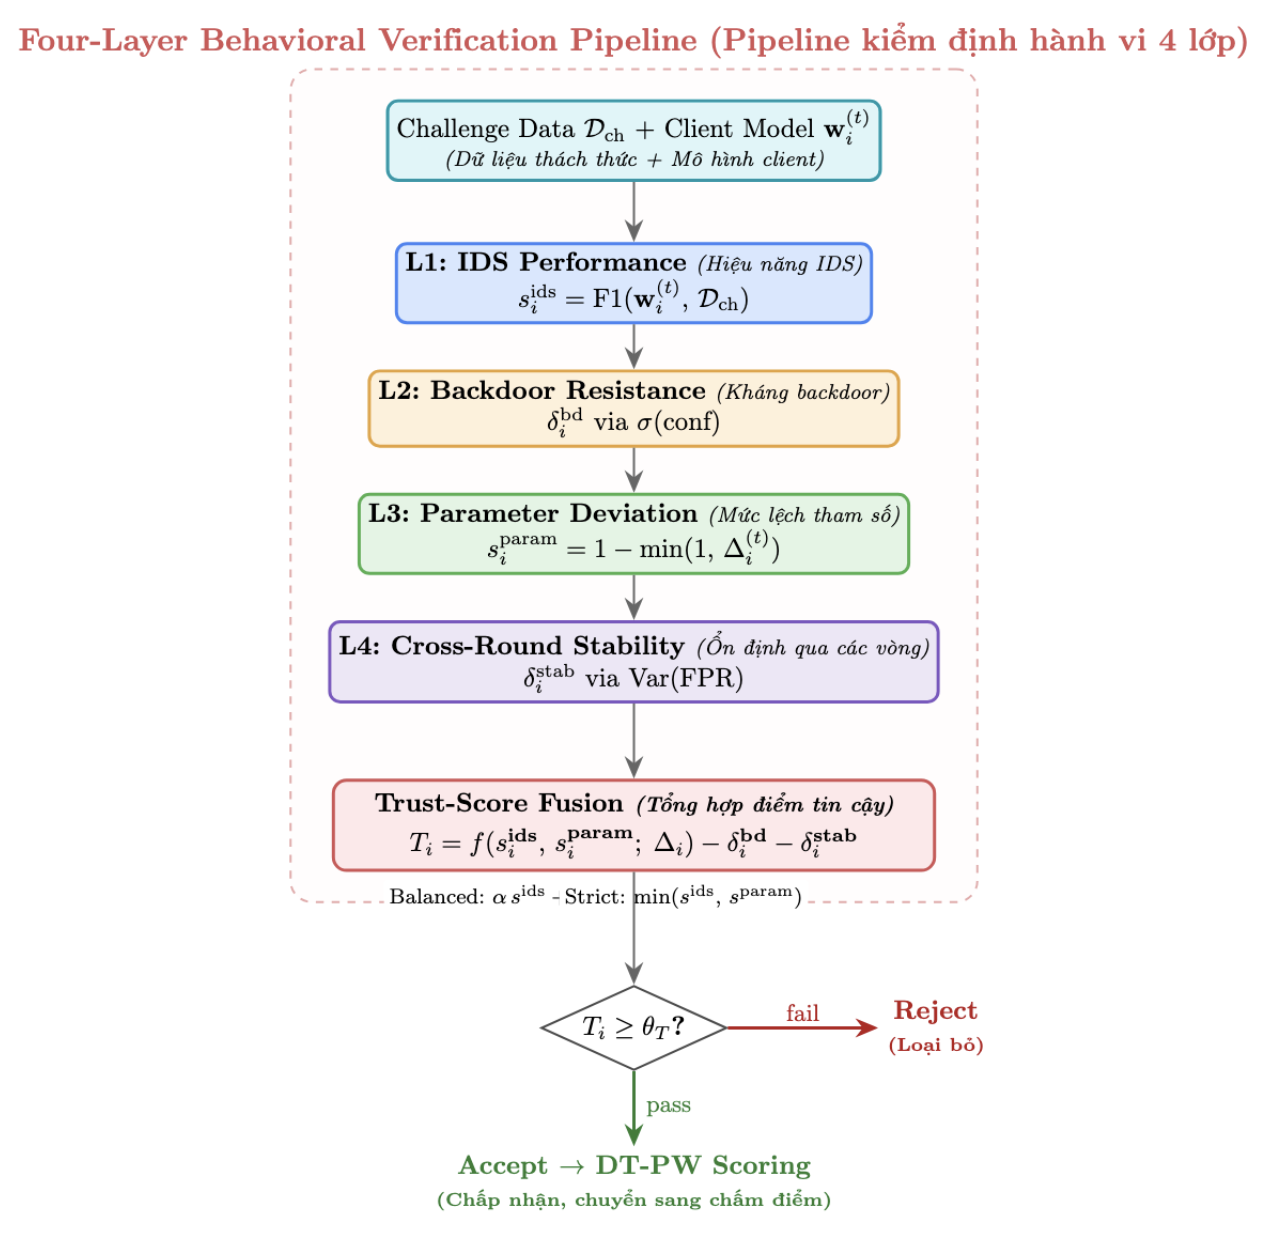
\includegraphics[width=0.85\linewidth]{Figures/fig_4_3_pipeline_kiem_dinh_4_lop.png}
    \caption{Pipeline kiểm định hành vi 4 lớp với Trust-Score}
\end{figure}

\subsection{Lớp 1: IDS Performance Score}
Lớp đầu tiên đánh giá trực tiếp năng lực phát hiện xâm nhập của mô hình cục bộ trên dữ liệu thách thức. Mô hình $\mathbf{w}_{i}^{(t)}$ được nạp vào sandbox, chạy inference trên toàn bộ $D_{\text{ch}}$, và được chấm điểm bằng F1-Score (phân loại nhị phân benign vs. attack):

\begin{equation}
s_{i}(\text{ids}) = F1(\mathbf{w}_{i}^{(t)},D_{\text{ch}}) \in \lbrack 0,1\rbrack
\tag{4.1}
\end{equation}

Trong đó: $s_{i}(ids)$ là IDS Performance Score của client i; F1($\cdot,\cdot)$ là F1-Score phân loại nhị phân (benign vs. attack); $\mathbf{w}_{i}^{(t)}$ là tham số mô hình cục bộ của client i tại round t; $D_{\text{ch}}$ là bộ dữ liệu thách thức gồm M mẫu.

F1-Score được chọn thay vì Accuracy vì cân bằng giữa Precision và Recall, phù hợp cho bài toán mất cân bằng lớp trong IDS. Mô hình lành tính (dù tham số lệch do Non-IID) vẫn đạt F1 cao vì đã thực sự học tri thức IDS hữu ích. Mô hình bị đầu độc có F1 thấp do phân loại sai trên các lớp tấn công mà nó bị nhắm đến.

Đây là lớp quan trọng nhất trong pipeline vì đánh giá trực tiếp năng lực suy luận của mô hình thay vì chỉ xem xét tham số. Các tấn công như LIE hay Min-Max có thể giữ tham số trong vùng bình thường, nhưng khi phải phân loại trên $D_{\text{ch}}$, hiệu năng thực tế sẽ suy giảm rõ rệt, kéo $s_{i}(ids)$ xuống thấp. Ngược lại, client Non-IID lành tính có tham số lệch nhưng vẫn phân loại chính xác, nên $s_{i}(ids)$ vẫn cao.

\subsection{Lớp 2: Backdoor Resistance Score}
Lớp thứ hai nhắm đến tấn công backdoor, loại tấn công khó phát hiện nhất vì mô hình hoạt động bình thường trên dữ liệu sạch, chỉ sai khi gặp trigger. DT-Guard khai thác quan sát: mô hình nhiễm backdoor có phân phối confidence bất thường, khi gặp mẫu gần trigger, softmax confidence lệch mạnh so với bình thường.

Cụ thể, DT-Guard tính độ lệch chuẩn $\sigma(conf)$ của softmax confidence trên $D_{\text{ch}}$. Nếu $\sigma(conf)$ vượt ngưỡng $\tau_{\text{bd}}$ (ước lượng từ mô hình toàn cục làm chuẩn), mô hình bị phạt:

\begin{equation}
\delta_{i}(\text{bd}) = \begin{cases}
  \lambda_{\text{bd}} & \text{nếu }\sigma(\text{conf}(\mathbf{w}_{i}^{(t)},D_{\text{ch}})) > \tau_{\text{bd}} \\
  0 & \text{nếu ngược lại}
\end{cases}\
\tag{4.2}
\end{equation}

Trong đó: $\delta_{i}(bd)$ là Backdoor Penalty của client i; $\sigma(\cdot)$ là độ lệch chuẩn của softmax confidence trên $D_{\text{ch}}$; $\tau_{\text{bd}}$ là ngưỡng variance confidence (ước lượng từ mô hình toàn cục); $\lambda_{\text{bd}}$ là hệ số phạt. Mô hình sạch có confidence ổn định nên không bị phạt. Mô hình nhiễm backdoor có confidence dao động mạnh khi gặp các mẫu gần trigger nên bị phạt $\lambda_{\text{bd}}$.

Cách tiếp cận này không cần biết trước trigger pattern, điều không khả thi trong FL vì server không có quyền truy cập dữ liệu của client. Thay vào đó, DT-Guard phát hiện gián tiếp thông qua dấu hiệu bất thường trong phân phối confidence. Mô hình nhiễm backdoor phải duy trì đồng thời hai hành vi đối lập (phân loại đúng trên dữ liệu sạch và phân loại sai khi có trigger), điều này tạo ra phân phối confidence không tự nhiên mà lớp kiểm định này có thể nắm bắt.

\subsection{Lớp 3: Parameter Deviation Score}
Lớp thứ ba đánh giá mức lệch tham số của mô hình cục bộ so với mô hình toàn cục. DT-Guard tính trung bình khoảng cách L2 theo từng lớp (layer) của mô hình, chuẩn hóa bằng $D_{\max}$:

\begin{equation}
\Delta_{i}^{(t)} = \frac{1}{L} \cdot \sum_{l = 1}^{L}\frac{\left\| \mathbf{w}_{i,l}^{(t)} - \mathbf{w}_{l}^{\left( t-1 \right)} \right\|_{2}}{D_{\max}} \geq 0
\tag{4.3}
\end{equation}

Trong đó: $\Delta_{i}^{(t)}$ là mức lệch tham số chuẩn hóa của client i tại round t; L là số lớp (layer) trainable trong mô hình; $\mathbf{w}_{i,l}^{(t)}$ là tham số lớp $\ell$ của client i; $\mathbf{w}_{l}^{(t-1)}$ là tham số lớp $\ell$ của mô hình toàn cục round trước; $D_{\max}$ \textgreater 0 là hằng số chuẩn hóa. Giá trị $\Delta_{i}$ được ánh xạ sang điểm tương đồng:

\begin{equation}
s_{i}(\text{param}) = 1 - \min(1,\Delta_{i}^{(t)}) \in \lbrack 0,1\rbrack
\tag{4.4}
\end{equation}

Trong đó $s_{i}(param)$ là Parameter Similarity Score. Khi $\Delta_{i}$ \textgreater 1, tham số lệch vượt giới hạn chuẩn hóa, $s_{i}(param)$ = 0.

Cần lưu ý rằng lớp này không được sử dụng đơn lẻ để quyết định chấp nhận hay loại bỏ client, vì làm vậy sẽ gây FPR cao giống như Krum, GeoMed hay LUP. Thay vào đó, Parameter Deviation đóng vai trò thông tin bổ sung cho cơ chế fusion thích ứng ở Mục 4.4.5. Khi $\Delta_{i}$ cao, hệ thống tự động chuyển sang strict mode, đồng thời yêu cầu $s_{i}(ids)$ cũng phải đạt mức cao. Nhờ vậy, DT-Guard phân biệt được client Non-IID lành tính ($\Delta_{i}$ cao nhưng $s_{i}(ids)$ cao vì phân loại đúng) với client độc hại ($\Delta_{i}$ cao và $s_{i}(ids)$ thấp vì phân loại sai).

\subsection{Lớp 4: Cross-Round Stability Score}
Lớp thứ tư phát hiện hành vi bất ổn định qua các vòng, dấu hiệu của attacker thay đổi chiến thuật liên tục hoặc mô hình bị nhiễu ngẫu nhiên. DT-Guard theo dõi FPR (False Positive Rate ở cấp traffic) của mỗi client qua cửa sổ trượt $\tau$ round gần nhất. Nếu variance vượt ngưỡng $\tau_{\text{stab}}$, client bị phạt:

\begin{equation}
\delta_{i}(\text{stab}) = \begin{cases}
  \lambda_{\text{stab}} & \text{nếu Var}(FPR_{i}^{\left( t-\tau \right)},\ldots,FPR_{i}^{(t)}) > \tau_{\text{stab}} \\
  0 & \text{nếu ngược lại}
\end{cases}\
\tag{4.5}
\end{equation}

Trong đó: $\delta_{i}(stab)$ là Stability Penalty của client i; Var($\cdot)$ là phương sai; $FPR_{i}^{(t)}$ là False Positive Rate ở cấp traffic của client i tại round t; $\tau$ là kích thước cửa sổ trượt; $\tau_{\text{stab}}$ là ngưỡng variance FPR; $\lambda_{\text{stab}}$ là hệ số phạt. Client mới (chưa đủ $\tau$ round lịch sử) được gán $\delta_{i}(stab)$ = 0 (không phạt).

Lớp này dựa trên quan sát rằng client lành tính có hành vi ổn định qua các round: FPR thay đổi ít. Trong khi đó, attacker thường thay đổi chiến thuật qua các vòng (ví dụ round trước sử dụng LIE, round sau chuyển sang Min-Max), tạo ra biến động lớn trong FPR và bị lớp kiểm định này phát hiện.

\subsection{Trust-Score Fusion}
Bốn lớp được tổng hợp thành Trust-Score duy nhất $T_{i}$ qua cơ chế fusion thích ứng. Trust-Score bao gồm điểm cơ bản trừ đi hai penalty:

\begin{equation}
T_{i} = f(s_{i}(\text{ids}),s_{i}(\text{param});\Delta_{i}^{(t)}) - \delta_{i}(\text{bd}) - \delta_{i}(\text{stab})
\tag{4.6}
\end{equation}

Trong đó hàm \emph{f}($\cdot)$ tổng hợp Lớp 1 và Lớp 3 theo cơ chế thích ứng hai chế độ dựa trên mức lệch tham số:

\[f( \cdot ) = \alpha \cdot s_{i}(\text{ids}) + (1 - \alpha) \cdot s_{i}(\text{param})\text{nếu }\Delta_{i}^{(t)} \leq \theta_{\text{div}}\text{(balanced mode)(4.7a)}\]

\[f( \cdot ) = \min(s_{i}(\text{ids}),s_{i}(\text{param}))\text{nếu }\Delta_{i}^{(t)} > \theta_{\text{div}}\text{(strict mode)(4.7b)}\]

Trong đó: $\alpha$ $\in$ {[}0, 1{]} là trọng số cân bằng giữa hiệu năng IDS và tương đồng tham số; $\theta_{\text{div}}$ \textgreater 0 là ngưỡng chuyển chế độ.

Balanced mode ($\Delta_{i}$ $\leq$ $\theta_{\text{div}}$): Tham số lệch ít, khả năng cao là client bình thường. Hệ thống sử dụng kết hợp tuyến tính với $\alpha$ = 0,7, ưu tiên IDS Performance (đánh giá hành vi trực tiếp) hơn Parameter Similarity (thông tin gián tiếp). Chế độ này cho phép client Non-IID có $s_{i}(param)$ trung bình nhưng $s_{i}(ids)$ cao vẫn đạt Trust-Score tốt.

Strict mode ($\Delta_{i}$ \textgreater $\theta_{\text{div}}$): Tham số lệch nhiều, cần kiểm tra nghiêm ngặt. Hệ thống lấy min: cả $s_{i}(ids)$ và $s_{i}(param)$ phải đồng thời cao. Client độc hại dù giữ $s_{i}(param)$ trung bình (qua tối ưu ngược) nhưng $s_{i}(ids)$ thấp $\rightarrow$ min thấp $\rightarrow$ bị loại. Client Non-IID lành tính có $\Delta_{i}$ cao nhưng $s_{i}(ids)$ cũng cao (phân loại đúng trên challenge data) $\rightarrow$ min vẫn đủ cao.

Sau khi tính $T_{i},$ client chỉ được chấp nhận khi $T_{i}$ $\geq$ $\theta_{T}$ ($\theta_{T}$ = 0,6 cho CIC-IoT-2023, $\theta_{T}$ = 0,5 cho ToN-IoT). Tập client vượt qua Trust Gate gọi là $\mathcal{T}$.

\begin{longtable}[]{@{}
  >{\raggedright\arraybackslash}p{(\linewidth - 4\tabcolsep) * \real{0.1474}}
  >{\raggedright\arraybackslash}p{(\linewidth - 4\tabcolsep) * \real{0.3669}}
  >{\raggedright\arraybackslash}p{(\linewidth - 4\tabcolsep) * \real{0.4857}}@{}}
\caption{Bảng tổng hợp tham số Trust Gate} \\
\toprule\noalign{}
\begin{minipage}[b]{\linewidth}\centering
\textbf{Tham số}
\end{minipage} & \begin{minipage}[b]{\linewidth}\centering
\textbf{Giá trị}
\end{minipage} & \begin{minipage}[b]{\linewidth}\centering
\textbf{Ý nghĩa}
\end{minipage} \\
\midrule\noalign{}
\endfirsthead
%
\multicolumn{3}{c}{{\textit{(tiếp) Bảng 4.2}}} \\
\toprule\noalign{}
\begin{minipage}[b]{\linewidth}\centering
\textbf{Tham số}
\end{minipage} & \begin{minipage}[b]{\linewidth}\centering
\textbf{Giá trị}
\end{minipage} & \begin{minipage}[b]{\linewidth}\centering
\textbf{Ý nghĩa}
\end{minipage} \\
\midrule\noalign{}
\endhead
\bottomrule\noalign{}
\endlastfoot
$\alpha$ & 0,7 & Tỉ trọng IDS Performance trong balanced mode \\
$\theta_{\text{div}}$ & Tùy chỉnh & Ngưỡng chuyển balanced $\rightarrow$ strict mode \\
$\lambda_{\text{bd}}$ & Tùy chỉnh & Hệ số phạt backdoor \\
$\lambda_{\text{stab}}$ & Tùy chỉnh & Hệ số phạt bất ổn định \\
$\theta_{T}$ & 0,6 (CIC-IoT-2023) / 0,5 (ToN-IoT) & Ngưỡng chấp nhận Trust-Score \\
$D_{\max}$ & 0 & Hằng số chuẩn hóa khoảng cách tham số \\
\end{longtable}

\section{Cơ chế DT-PW với Effort Gate}
Cơ chế DT-Driven Performance Weighting (DT-PW) giải quyết Khoảng trống 3: thiếu cơ chế đo đóng góp tri thức thực tế và vấn đề free-rider. Sau khi client vượt qua Trust Gate (tập $\mathcal{T}),$ DT-PW tiếp tục đánh giá mức đóng góp tri thức mới của từng client.

\begin{figure}[H]
    \centering
    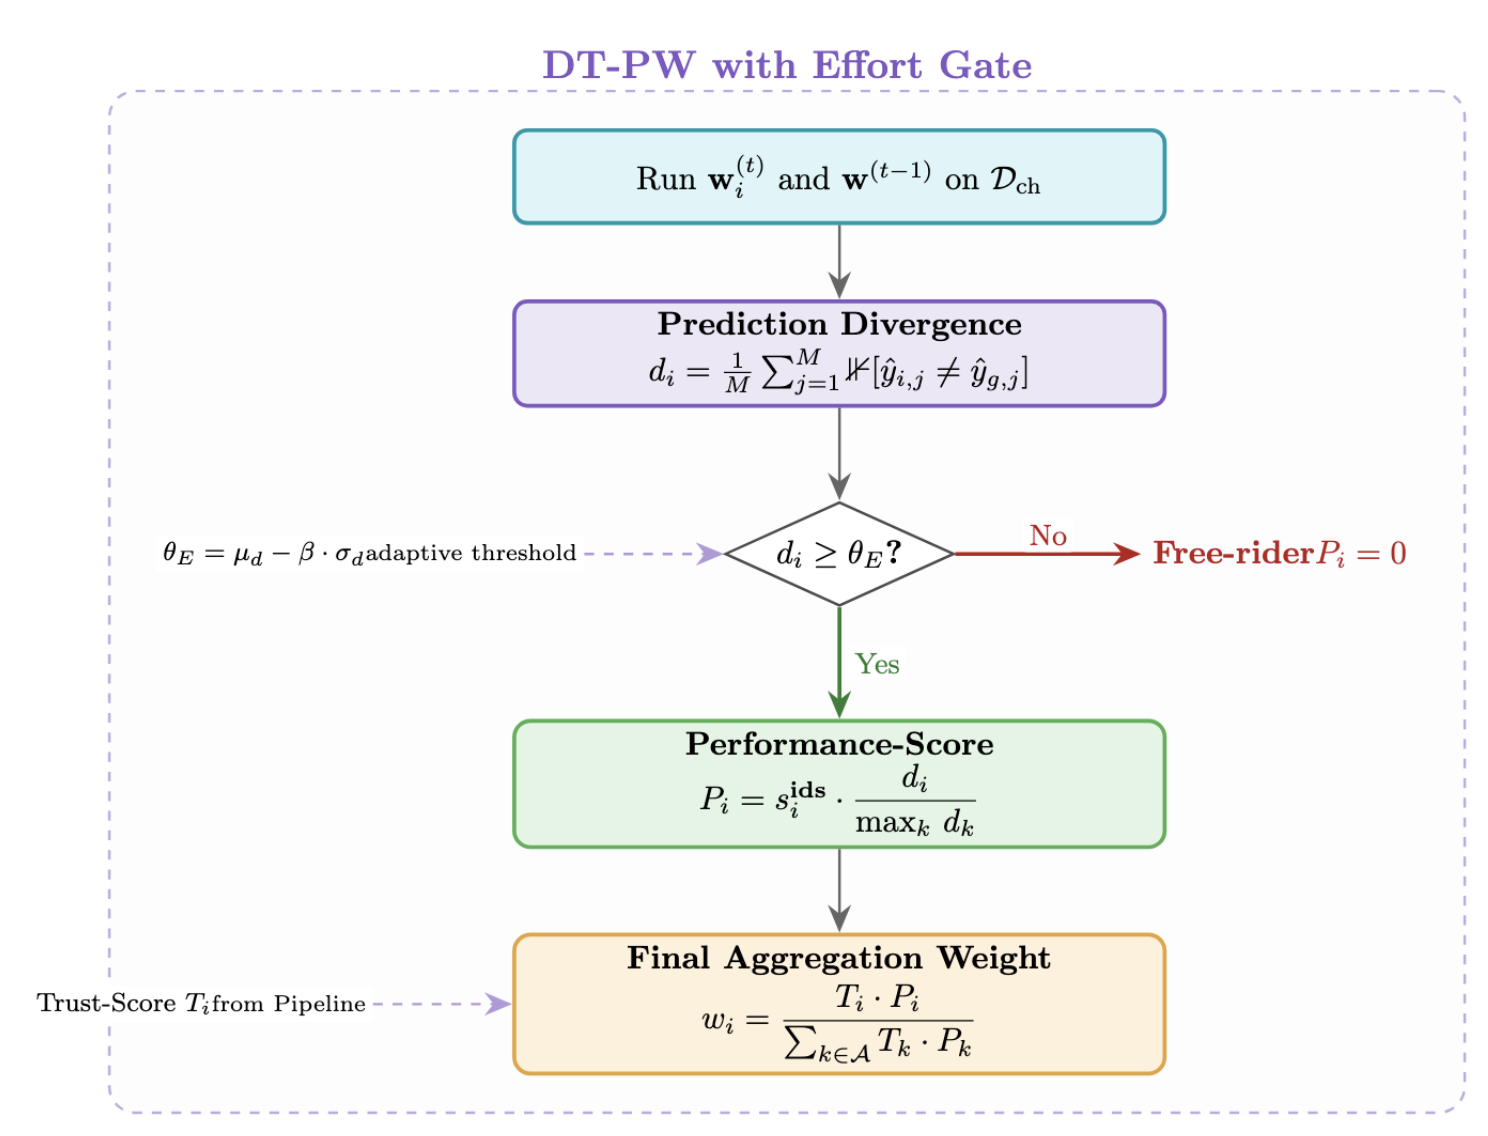
\includegraphics[width=0.85\linewidth]{Figures/fig_4_4_co_che_dtpw_effort_gate.png}
    \caption{Cơ chế DT-PW với Effort Gate}
\end{figure}

\subsection{Prediction Divergence}
Ý tưởng cốt lõi: client thực sự huấn luyện trên dữ liệu riêng sẽ học được tri thức mới mà mô hình toàn cục chưa có, dẫn đến dự đoán khác biệt trên $D_{\text{ch}}$. Free-rider chỉ sao chép $\mathbf{w}^{(t-1)}$ kèm nhiễu nhỏ, dự đoán gần như y hệt.

Cả $\mathbf{w}_{i}^{(t)}$ và $\mathbf{w}^{(t-1)}$ được nạp vào sandbox, chạy inference trên $D_{\text{ch}}$. Prediction divergence $d_{i}$ đo tỉ lệ mẫu có dự đoán khác nhau:

\begin{equation}
d_{i} = \frac{1}{M} \cdot \sum_{j = 1}^{M}\mathbb{1}\lbrack{\overset{\hat{}}{y}}_{i,j} \neq {\overset{\hat{}}{y}}_{g,j}\rbrack
\tag{4.8}
\end{equation}

Trong đó M = $|D_{\text{ch}}|$ là số mẫu, $\hat y_{i,j}$ = argmax $\mathbf{w}_{i}^{(t)}(x_{j})$ là dự đoán của mô hình cục bộ, $\hat y_{g,j}$ = argmax $\mathbf{w}^{(t-1)}(x_{j})$ là dự đoán của mô hình toàn cục, và $\mathbb{1}${[}$\cdot${]} là hàm chỉ thị (indicator function). Giá trị $d_{i}$ $\in$ {[}0, 1{]}:

\begin{itemize}
\item
  $d_{i}$ $\approx$ 0: Mô hình cục bộ dự đoán gần như y hệt mô hình toàn cục $\rightarrow$ free-rider.
\item
  $d_{i}$ \textgreater{} 0: Mô hình cục bộ có tri thức khác biệt $\rightarrow$ đã thực sự huấn luyện.
\end{itemize}

\subsection{Effort Gate}
Effort Gate phân biệt free-rider với client đóng góp thực sự bằng ngưỡng thích ứng. Ngưỡng $\theta_{E}$ được tính động dựa trên phân phối $\{d_{i}\}_{i\in\mathcal{T}}$ của tập client đã qua Trust Gate:

\begin{equation}
\theta_{E} = \mu_{d} - \beta \cdot \sigma_{d}
\tag{4.9}
\end{equation}

Trong đó $\mu_{d}$ = mean($\{d_{i}\}_{i\in\mathcal{T}}$) là trung bình, $\sigma_{d}$ = std($\{d_{i}\}_{i\in\mathcal{T}}$) là độ lệch chuẩn, và $\beta$ \textgreater 0 kiểm soát độ nhạy. $\beta$ lớn $\rightarrow$ ngưỡng thấp $\rightarrow$ ít client bị coi là free-rider; $\beta$ nhỏ $\rightarrow$ ngưỡng cao $\rightarrow$ nghiêm ngặt hơn.

Cơ chế ngưỡng thích ứng này quan trọng vì mức divergence "bình thường" thay đổi theo từng round (phụ thuộc vào mức hội tụ hiện tại, phân bổ dữ liệu, và loại tấn công). Thay vì dùng ngưỡng cố định (dễ quá nhạy hoặc quá lỏng), Effort Gate tự điều chỉnh dựa trên phân phối thực tế của round hiện tại.

Quyết định:

\begin{itemize}
\item
  Nếu $d_{i}$ \textless{} $\theta_{E}$: Client bị xem là free-rider $\rightarrow$ $P_{i}$ = 0.
\item
  Nếu $d_{i}$ $\geq$ $\theta_{E}$: Client được xem là đóng góp thực chất $\rightarrow$ được chấm Performance-Score.
\end{itemize}

\subsection{Performance-Score}
Đối với client vượt qua Effort Gate ($d_{i}$ $\geq$ $\theta_{E}$), Performance-Score kết hợp hai yếu tố: năng lực phát hiện xâm nhập (qua $s_{i}(ids)$ đã tính ở Lớp 1) và mức đóng góp tri thức mới (qua $d_{i}$ chuẩn hóa):

\begin{equation}
P_{i} = s_{i}(\text{ids}) \cdot \frac{d_{i}}{\max_{k}d_{k}}
\tag{4.10}
\end{equation}

Trong đó $max_{k}$ $d_{k}$ chuẩn hóa divergence về {[}0, 1{]}. Công thức đảm bảo: client có $s_{i}(ids)$ cao VÀ $d_{i}$ cao mới đạt $P_{i}$ cao. Client chỉ diverge nhiều nhưng phân loại kém (có thể do nhiễu) sẽ bị $s_{i}(ids)$ thấp kéo $P_{i}$ xuống.

\subsection{Trọng số tổng hợp cuối cùng}
Trọng số tổng hợp cho mỗi client kết hợp cả Trust-Score (độ tin cậy) và Performance-Score (mức đóng góp):

\begin{equation}
w_{i} = \frac{T_{i} \cdot P_{i}}{\sum_{k \in \mathcal{A}}^{}(T_{k} \cdot P_{k})}
\tag{4.11}
\end{equation}

Trong đó $\mathcal{A}$ là tập client được chấp nhận (qua cả Trust Gate và Effort Gate, có $P_{i}$ \textgreater 0). Mô hình toàn cục mới:

\begin{equation}
\mathbf{w}^{(t)} = \sum_{i \in \mathcal{A}}^{}w_{i} \cdot \mathbf{w}_{i}^{(t)}
\tag{4.12}
\end{equation}

Tính chất của công thức tổng hợp:

\begin{itemize}
\item
  Client bị Trust Gate loại ($T_{i}$ \textless{} $\theta_{T}$): Không thuộc $\mathcal{A},$ trọng số = 0.
\item
  Client bị Effort Gate loại ($d_{i}$ \textless{} $\theta_{E}$): $P_{i}$ = 0 $\rightarrow$ $w_{i}$ = 0.
\item
  Client đáng tin nhưng không đóng góp (free-rider): $T_{i}$ cao nhưng $P_{i}$ = 0 $\rightarrow$ $w_{i}$ = 0.
\item
  Client đóng góp nhưng không đáng tin (poisoner qua được Effort Gate): $P_{i}$ \textgreater{} 0 nhưng $T_{i}$ thấp $\rightarrow$ $w_{i}$ nhỏ.
\item
  Client vừa đáng tin vừa đóng góp: $T_{i}$ cao VÀ $P_{i}$ cao $\rightarrow$ $w_{i}$ lớn.
\end{itemize}

\section{Phân tích lý thuyết}

\subsection{Tại sao kiểm chứng hành vi vượt trội phân tích tham số thụ động}
Lợi thế của active behavioral verification có thể được phân tích qua bốn trường hợp điển hình:

Trường hợp 1 (Tấn công LIE {[}1{]}): LIE tạo tham số độc hại bằng cách cộng một lượng nhỏ vào giá trị trung bình của các bản cập nhật lành tính, giữ tham số trong vùng phân phối bình thường nên Krum, Median, GeoMed không phát hiện. Tuy nhiên, khi chạy trên challenge data, mô hình phân loại sai trên các lớp tấn công $\rightarrow$ điểm IDS Performance thấp $\rightarrow$ Trust Gate loại bỏ.

Trường hợp 2 (Tấn công Min-Max/Min-Sum {[}15{]}): Attacker tối ưu hóa bản cập nhật độc hại sao cho khoảng cách đến các update lành tính nằm trong giới hạn cho phép nên các bộ lọc khoảng cách thất bại. Nhưng hành vi phân loại bộc lộ trên challenge data $\rightarrow$ điểm IDS Performance thấp $\rightarrow$ bị loại.

Trường hợp 3 (Client Non-IID lành tính): Tham số của client lệch xa mô hình toàn cục do dữ liệu thiên lệch nên các phương pháp thụ động nhầm là tấn công (FPR cao). Nhưng mô hình vẫn phân loại chính xác trên challenge data (cân bằng nhãn) $\rightarrow$ điểm IDS Performance cao $\rightarrow$ vượt Trust Gate. Trong balanced mode, điểm IDS Performance cao (trọng số 0,7) bù cho điểm Parameter Similarity thấp (trọng số 0,3), đạt FPR = 0\%.

Trường hợp 4 (Free-rider): Tham số của free-rider gần như trùng với mô hình toàn cục (chỉ thêm nhiễu nhỏ) nên Trust-Score (LUP) thưởng 0,2448 (thực nghiệm). Nhưng prediction divergence gần bằng 0 $\rightarrow$ Effort Gate phát hiện $\rightarrow$ Performance-Score bằng 0 $\rightarrow$ trọng số = 0.

\subsection{Đảm bảo an toàn với sandbox isolation}
Digital Twin Sandbox cung cấp ba lớp đảm bảo an toàn:

\textbf{(1) Cách ly thực thi:} Mô hình được nạp vào sandbox dưới dạng bản sao tham số trên vùng nhớ riêng. Mọi thao tác (inference, gradient computation nếu có) chỉ ảnh hưởng đến vùng nhớ sandbox, không tác động đến FL Server hay mô hình toàn cục.

\textbf{(2) Reset sau kiểm chứng:} Sau mỗi lần kiểm tra, sandbox giải phóng toàn bộ tensor và context liên quan đến mô hình vừa kiểm tra, reset về trạng thái sạch trước khi nạp mô hình tiếp theo. Điều này ngăn chặn tấn công khai thác trạng thái tồn đọng.

\textbf{(3) Sequential loading:} Sandbox chỉ nạp một mô hình tại một thời điểm, giải phóng trước khi nạp mô hình kế tiếp. Cơ chế này vừa đảm bảo an toàn vừa tối ưu bộ nhớ, giúp peak memory thấp hơn cả FedAvg (phải giữ tất cả N bản cập nhật đồng thời).

\subsection{Độ phức tạp tính toán}
Chi phí tính toán bổ sung của DT-Guard mỗi round gồm hai thành phần:

\textbf{(1) Trust verification:} O(M $\times$ N), với M = $|D_{\text{ch}}|$ là số mẫu challenge data và N là số client. Mỗi client cần chạy inference M mẫu qua mạng IDS.

\textbf{(2) DT-PW scoring:} O(M $\times$ N), cần chạy inference cả mô hình cục bộ lẫn mô hình toàn cục trên M mẫu, rồi so sánh M cặp dự đoán.

Tổng overhead: O(M $\times$ N), được tối ưu nhờ pre-generated challenge pool (không sinh dữ liệu mới mỗi round) và sequential model loading. Thực nghiệm cho thấy overhead chiếm dưới 1\% tổng thời gian round.

\section{Tổng kết chương}
Chương này đã trình bày kiến trúc DT-Guard gồm năm thành phần chính: kiến trúc tổng thể 3 thực thể, bộ sinh TabDDPM, pipeline kiểm định 4 lớp với Trust-Score (Công thức 4.1--4.7), cơ chế DT-PW với Effort Gate (Công thức 4.8--4.12), và phân tích lý thuyết. Chương tiếp theo trình bày thực nghiệm và đánh giá trên hai bộ dữ liệu CIC-IoT-2023 và ToN-IoT.
